%!TEX program = xelatex
\documentclass[aspectratio=169,10pt]{ctexbeamer}
\usetheme{fduclassroom}

\usepackage[UTF8,fontset=none]{ctex}
\usepackage{amsmath,amssymb,mathtools,bm}
\usepackage{booktabs,array,tabularx}
\usepackage{tikz,pgfplots}
\usetikzlibrary{arrows.meta,calc,positioning}
\pgfplotsset{compat=1.18}
\usepackage{hyperref}
\usepackage{pgfplots}
\pgfplotsset{compat=1.17}

\IfFontExistsTF{TeX Gyre Heros}{\setsansfont{TeX Gyre Heros}}{}
\IfFontExistsTF{PingFang SC}{
  \setCJKmainfont{PingFang SC}
  \setCJKsansfont{PingFang SC}
}{
  \setCJKmainfont{SimSun}
  \setCJKsansfont{SimHei}
}
\usefonttheme{professionalfonts}

\newcommand{\RR}{\mathbb{R}}
\newcommand{\NN}{\mathbb{N}}
\newcommand{\eps}{\varepsilon}
\newcommand{\term}[1]{\textcolor{FDUBlue}{\bfseries #1}}
\newcommand{\warn}[1]{\textcolor{FDURed}{\bfseries #1}}
\newcommand{\source}[1]{\par\vfill{\tiny\color{MutedText}资料来源：#1}}
\newcommand{\qedhereppt}{\hfill$\square$}
\newcommand{\sectionframe}{\begin{frame}[plain]\sectionpage\end{frame}}
\newcolumntype{Y}{>{\raggedright\arraybackslash}X}
\newcommand{\ee}{\mathrm{e}}

% --- 自动生成带进度颜色的章节过渡页 ---
\AtBeginSection[]{
	\begin{frame}{目录}
		% 临时重定义目录中 section 的排版格式
		\setbeamertemplate{section in toc}{%
			\leavevmode\leftskip=2em % 整体向右缩进一点使其居中对齐
			\ifnum\inserttocsectionnumber>\insertsectionnumber\relax
			% 1. 未来的章节（大于当前章节号）：使用 MutedText（浅灰色）
			\color{MutedText}%
			\else
			\ifnum\inserttocsectionnumber=\insertsectionnumber\relax
			% 2. 当前即将开始的章节：使用 FDUBlue 并加粗（高亮深色）
			\color{FDUBlue}\bfseries%
			\else
			% 3. 已经结束的章节（过去）：使用 TextBlack（普通深色）
			\color{TextBlack}%
			\fi
			\fi
			% 输出章节号和章节名称
			% 【修改此处】：将原来的 \vspace{0.3cm} 改小，例如改为 0.1cm 或 0.15cm
			\inserttocsectionnumber. \inserttocsection\par\vspace{0.1cm}
		}
		
		% 生成目录，并隐藏子章节(subsection)以保持过渡页清爽
		\tableofcontents[hideallsubsections]
	\end{frame}
}

\addtobeamertemplate{frametitle}{\vspace*{0.5cm}}{}
\title[第三章：函数极限与连续性]{第三章：函数极限与连续性}
\author[大学数学（I）]{大学数学（I）}

\begin{document}

\begin{frame}[plain]
  \titlepage
\end{frame}






\section{一元函数极限}



\begin{frame}{$x\to x_0$时的函数极限}

	
	\begin{block}{定义}
	设函数 \(f\) 在点 \(x_0\) 的某个去心邻域内有定义。若存在常数 \(A\)，使得对任意 \(\varepsilon>0\)，总存在 \(\delta>0\)，当
	\[
	0<|x-x_0|<\delta
	\]
	时都有
	\[
	|f(x)-A|<\varepsilon,
	\]
	则称当 \(x\to x_0\) 时 \(f(x)\) 的极限为 \(A\)，记作
	\[
	\lim\limits_{x\to x_0}f(x)=A.
	\]
	\end{block}

\end{frame}

\begin{frame}{按定义证明函数极限}
	\begin{block}{例题}
	证明
	\[
	\lim\limits_{x\to2}(3x-1)=5.
	\]
	\end{block}
	\pause
	\textbf{证明：}
	
	任取 \(\varepsilon>0\)。注意到
	\[
	|(3x-1)-5|=3|x-2|.
	\]
	取 \(\delta=\varepsilon/3\)，则当 \(0<|x-2|<\delta\) 时，
	\[
	|(3x-1)-5|<3\delta=\varepsilon.
	\]
	因此 \(\lim\limits_{x\to2}(3x-1)=5\)。
	

	
\end{frame}

\begin{frame}{极限与函数在该点的取值无关}
	\begin{block}{ }
		函数极限只考察去心邻域，所以 \(f(x_0)\) 可以等于极限、不同于极限，甚至没有定义。例如
		\[
		f(x)=
		\begin{cases}
			\dfrac{x^2-1}{x-1},&x\neq1,\\
			100,&x=1
		\end{cases}
		\]
		满足 \(\lim\limits_{x\to1}f(x)=2\)，尽管 \(f(1)=100\)。改变单独一个点的函数值不会改变该点的极限。
	\end{block}
\end{frame}


\begin{frame}{$x\to \infty  $时的函数极限}
	\begin{block}{定义}
		设有函数 $f(x)$ 和常数 $A$ ，如果对任意给定的 $\varepsilon>0$ ，存在 $X>0$ ，使当 $|x|>X$ 时，总有不等式
		
		$$
		|f(x)-A|<\varepsilon
		$$
		
		成立，则称常数 $A$ 为 $x \rightarrow \infty$ 时函数 $f(x)$ 的极限，记为
		
		$$
		\lim\limits _{x \to \infty} f(x)=A \text {, 或 } f(x) \rightarrow A \quad(x \rightarrow \infty) \text {. }
		$$
	\end{block}    
\end{frame}

\begin{frame}{}
	\begin{block}{例题}
		用定义证明 $\lim\limits _{x \rightarrow \infty} \frac{2 x-1}{x}=2$ ．
		
	\end{block}
	
	\pause
	
	
	\vspace{0.3cm}
	
	\textbf{证明：}
	
	对于任意给定的 $\varepsilon>0$ ，要使
	
	$$
	|f(x)-2|=\left|\frac{2 x-1}{x}-2\right|=\frac{1}{|x|}<\varepsilon
	$$
	
	成立，只需 $|x|>\frac{1}{\varepsilon}$ ．因此，取 $X=\frac{1}{\varepsilon}$ ，则当 $|x|>X$ 时，必有
	
	$$
	|f(x)-2|=\left|\frac{2 x-1}{x}-2\right|<\varepsilon .
	$$
	
	于是，根据定义有
	
	$$
	\lim\limits _{x \rightarrow \infty} \frac{2 x-1}{x}=2 .
	$$
\end{frame}



\begin{frame}{左极限与右极限}
	\begin{block}{定义}
		若对任意 \(\varepsilon>0\)，存在 \(\delta>0\)，使得当 \(x_0-\delta<x<x_0\) 时，
		\[
		|f(x)-A|<\varepsilon,
		\]
		则称 \(A\) 为 \(f(x)\) 在 \(x_0\) 处的左极限，记作
		\[
		\lim\limits_{x\to x_0^-}f(x)=A.
		\]
		类似地，当 \(x_0<x<x_0+\delta\) 时满足上述不等式，则称 \(A\) 为右极限，记作
		\[
		\lim\limits_{x\to x_0^+}f(x)=A.
		\]
	\end{block}
\end{frame}

\begin{frame}{单侧极限与双侧极限}
	\footnotesize
	\begin{block}{双侧极限存在的充要条件}
		\[
		\lim\limits_{x\to x_0}f(x)=A
		\]
		当且仅当
		\[
		\lim\limits_{x\to x_0^-}f(x)=\lim\limits_{x\to x_0^+}f(x)=A.
		\]
	\end{block}
	若左右极限不相等，则会导致单侧极限存在而双侧极限不存在。
	
	\begin{block}{左右极限不相等的例子}
		设
		\[
		f(x)=
		\begin{cases}
			-1,&x<0,\\
			1,&x\geq0.
		\end{cases}
		\]
		\[
		\lim\limits_{x\to0^-}f(x)=-1,\qquad
		\lim\limits_{x\to0^+}f(x)=1.
		\]
		左右极限不相等，所以 \(\lim\limits_{x\to0}f(x)\) 不存在。
	\end{block}
\end{frame}


\begin{frame}{自变量趋于无穷时的有限极限}
	\small	
	\begin{block}{定义}
		若对任意 \(\varepsilon>0\)，存在 \(X>0\)，使得当 \(x>X\) 时都有
		\[
		|f(x)-A|<\varepsilon,
		\]
		则称 \(\lim\limits_{x\to+\infty}f(x)=A\)。将条件改为 \(x<-X\)，便得到 \(\lim\limits_{x\to-\infty}f(x)=A\) 的定义。
	\end{block}
	\pause
	
	\begin{block}{例子}
		\[
		\lim\limits_{x\to+\infty}\frac{2x+1}{x+3}=2.
		\]
		事实上，
		\[
		\left|\frac{2x+1}{x+3}-2\right|=\frac5{x+3}.
		\]
		给定 \(\varepsilon>0\)，取 \(X>\max\{0,5/\varepsilon-3\}\)，当 \(x>X\) 时上式小于 \(\varepsilon\)。
	\end{block}
\end{frame}




\section{函数极限的基本性质}


\begin{frame}{极限的唯一性}
	\begin{block}{性质1}
		若 \(\lim\limits_{x\to x_0}f(x)\) 存在，则其极限值唯一。
	\end{block}
	
	\textbf{证明：}
	
	假设 \(f(x)\) 同时以 \(A\) 和 \(B\) 为极限，且 \(A\neq B\)。取
	\[
	\varepsilon=\frac{|A-B|}{3}.
	\]
	当 \(x\) 充分接近 \(x_0\) 且 \(x\neq x_0\) 时，同时有
	\[
	|f(x)-A|<\varepsilon,\qquad |f(x)-B|<\varepsilon.
	\]
	由三角不等式，
	\[
	|A-B|\leq |A-f(x)|+|f(x)-B|<2\varepsilon=\frac23|A-B|,
	\]
	矛盾。因此 \(A=B\)。
	
	
\end{frame}

\begin{frame}{局部有界性与保号性}
	\begin{block}{性质2}
		若 \(\lim\limits_{x\to x_0}f(x)=A\)，则 \(f\) 在 \(x_0\) 的某个去心邻域内有界。若 \(A>0\)，则在某个去心邻域内 \(f(x)>0\)；若 \(A<0\)，则在某个去心邻域内 \(f(x)<0\)。
	\end{block}
	
	\textbf{证明：}
	
	在极限定义中取 \(\varepsilon=1\)，当 \(x\) 充分接近 \(x_0\) 时有
	\[
	|f(x)|\leq |f(x)-A|+|A|<1+|A|,
	\]
	故 \(f\) 局部有界。若 \(A>0\)，取 \(\varepsilon=A/2\)，则
	\[
	f(x)>A-\frac A2=\frac A2>0.
	\]
	\(A<0\) 的情形同理。
\end{frame}

\begin{frame}{四则运算法则}
	\normalsize
	\begin{block}{性质3}
		若 \(\lim\limits_{x\to x_0}f(x)=A\)，\(\lim\limits_{x\to x_0}g(x)=B\)，则
		\[
		\lim\limits_{x\to x_0}[f(x)\pm g(x)]=A\pm B,\qquad
		\lim\limits_{x\to x_0}f(x)g(x)=AB.
		\]
		若 \(B\neq0\)，则
		\[
		\lim\limits_{x\to x_0}\frac{f(x)}{g(x)}=\frac AB.
		\]
	\end{block}
\end{frame}

\begin{frame}{夹逼定理}
	\normalsize
	\begin{block}{性质4}
		若在 \(x_0\) 的某个去心邻域内
		\[
		g(x)\leq f(x)\leq h(x),
		\]
		且
		\[
		\lim\limits_{x\to x_0}g(x)=\lim\limits_{x\to x_0}h(x)=A,
		\]
		则 \(\lim\limits_{x\to x_0}f(x)=A\)。
	\end{block}
\end{frame}

\section{两个重要极限}



\begin{frame}{第一个重要极限}
	\begin{block}{ }
		\[
		\lim\limits_{x \to 0} \frac{\sin x}{x} = 1.
		\]
		
	\end{block}
	
	
	
		\begin{columns}[c] % [c] 表示左右两列垂直居中对齐，如果想顶部对齐可以改为 [T]
			
			% ========== 左侧列：放置图形 ==========
			\begin{column}{0.4\textwidth}
				\begin{center}
					% 注意：这里改成了 \textwidth，表示让图片占满这“0.4倍列宽”的全部空间
					\resizebox{0.7\textwidth}{!}{
						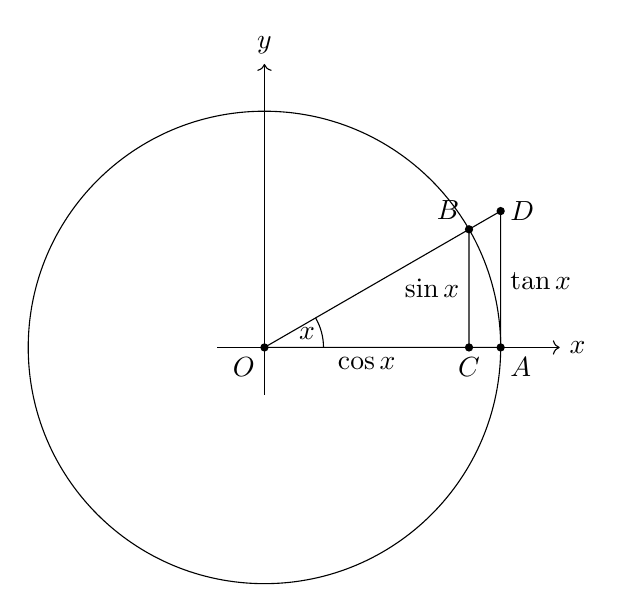
\begin{tikzpicture}[scale=3]
							\coordinate (O) at (0,0);
							\coordinate (A) at (1,0);
							\coordinate (B) at ({cos(30)},{sin(30)});
							\coordinate (C) at ({cos(30)},0);
							\coordinate (D) at (1,{tan(30)});
							\draw[->] (-0.2,0) -- (1.25,0) node[right] {$x$};
							\draw[->] (0,-0.2) -- (0,1.2) node[above] {$y$};
							\draw (O) circle (1);
							\draw (O)--(A) (O)--(D) (B)--(C) (A)--(D);
							\fill (O) circle (0.5pt) node[below left] {$O$};
							\fill (A) circle (0.5pt) node[below right] {$A$};
							\fill (B) circle (0.5pt) node[above left] {$B$};
							\fill (C) circle (0.5pt) node[below] {$C$};
							\fill (D) circle (0.5pt) node[right] {$D$};
							\draw (0.25,0) arc (0:30:0.25);
							\node at (0.18,0.06) {$x$};
							\node[right] at (1,0.28) {$\tan x$};
							\node[left] at ({cos(30)},0.25) {$\sin x$};
							\node[below] at ({cos(30)/2},0) {$\cos x$};
						\end{tikzpicture}
					} 
				\end{center}
			\end{column}
			
			% ========== 右侧列：放置文字 ==========
			\begin{column}{0.6\textwidth}
				\small
				画一个半径为 1 的圆。在圆中取一个很小的角 \(x\)，如图：
				\begin{itemize}
					\item 角 \(x\) 对应的圆弧长 = \(x\)\\ （因为半径=1，弧长=半径×角度）
					\item 垂线 \(BC\) 的长度 = \(\sin x\)
					\item 水平线 \(OC\) 的长度 = \(\cos x\)
					\item 切线 \(AD\) 的长度 = \(\tan x\)
				\end{itemize}
				
				\vspace{0.5em} % 增加一点垂直间距让排版不那么拥挤
				从图中可以看出，三个面积之间有如下关系：
				
				% 使用 \small 可以稍微缩小公式字体，防止超出右侧边界
				\small 
				\[
				\triangle OAB \text{ 的面积 } < \text{扇形 } OAB \text{ 的面积 } < \triangle OAD \text{ 的面积}
				\]
			\end{column}
			
		\end{columns}

\end{frame}

\begin{frame}{面积比较}
	\begin{itemize}
		\item \(\triangle OAB\) 的面积 = \(\dfrac{1}{2} \times 1 \times \sin x = \dfrac{1}{2} \sin x\)
		\item 扇形 \(OAB\) 的面积 = \(\dfrac{1}{2} \times 1^2 \times x = \dfrac{x}{2}\)
		\item \(\triangle OAD\) 的面积 = \(\dfrac{1}{2} \times 1 \times \tan x = \dfrac{1}{2} \tan x\)
	\end{itemize}
	
	因此：
	
	\[
	\dfrac{1}{2} \sin x  <  \dfrac{x}{2} < \dfrac{1}{2} \tan x \qquad (0 < x < \dfrac{\pi}{2}).
	\]
	
	两边同时乘以 2，得到：
	
	\[
	\sin x  < x < \tan x.
	\]
\end{frame}


\begin{frame}{推导 \(\dfrac{\sin x}{x}\) 的夹逼不等式}
	由 \(x < \tan x = \dfrac{\sin x}{\cos x}\)，两边同时除以 \(\sin x > 0\)，得：
	
	\[
	\dfrac{x}{\sin x} < \dfrac{1}{\cos x} \quad \Longrightarrow \quad \cos x < \dfrac{\sin x}{x}.
	\]
	
	又由 \(\sin x < x\)，两边除以 \(x > 0\)，得：
	
	\[
	\dfrac{\sin x}{x} < 1.
	\]
	
	合起来：
	
	\[
	\cos x < \dfrac{\sin x}{x} < 1 \qquad (0 < x < \dfrac{\pi}{2}).
	\]
	
\end{frame}

\begin{frame}{用夹逼准则取极限}
	由 \(|\sin u|\leq|u|\)，有
	\[
	0\leq1-\cos x=2\sin^2\frac x2\leq\frac{x^2}{2},
	\]
	所以由夹逼定理可先得到 \(\lim\limits_{x\to0}\cos x=1\)。因此，当 \(x \to 0^+\) 时：
	
	\[
	\cos x \;\longrightarrow\; 1,\quad \dfrac{\sin x}{x} \;\longrightarrow\; 1.
	\]
	
	当 \(x\) 为负时（即 \(x \to 0^-\)），由于 \(\dfrac{\sin x}{x}\) 是偶函数（\(\sin(-x)/(-x) = \sin x / x\)），左右极限相等。因此：
	
	\[
	\lim\limits_{x \to 0} \dfrac{\sin x}{x} = 1.
	\]
\end{frame}

\begin{frame}{利用第一个重要极限求极限}
	\begin{block}{例题}
		求 \(\lim\limits_{x \to 0} \dfrac{\sin 2x}{x}\)。
	\end{block}
	
	\pause
	
	\vspace{0.4cm}
	
	\textbf{证明：}
	
	\[
	\dfrac{\sin 2x}{x} = 2 \cdot \dfrac{\sin 2x}{2x} \to 2 \cdot 1 = 2.
	\]
	
	
	
\end{frame}


\begin{frame}{第二个重要极限——数列形式}
	\normalsize
	\begin{block}{收敛到自然常数 e}
		\[
		\lim\limits_{n\to\infty} \left(1 + \dfrac{1}{n}\right)^n = \ee.
		\]
	\end{block}
	

	
	
\end{frame}


\begin{frame}{数列形式下第二个重要极限的证明}
		\textbf{证明分为两步：先证 \(\{a_n\}\) 单调递增，再证它有上界。}
	
	\noindent\textbf{第一步：证明单调递增}
	
	由二项式定理展开：
	\[
	a_n = \left(1+\dfrac{1}{n}\right)^n = \sum\limits_{k=0}^{n} C_n^k \dfrac{1}{n^k} = \sum_{k=0}^{n} \dfrac{1}{k!} \cdot \dfrac{n(n-1)\cdots(n-k+1)}{n^k}.
	\]
	其中 \(\dfrac{n(n-1)\cdots(n-k+1)}{n^k} = 1 \cdot \left(1-\dfrac{1}{n}\right) \cdots \left(1-\dfrac{k-1}{n}\right)\)。于是
	\[
	a_n = \sum_{k=0}^{n} \dfrac{1}{k!} \left(1-\dfrac{1}{n}\right)\left(1-\dfrac{2}{n}\right)\cdots\left(1-\dfrac{k-1}{n}\right).
	\]
\end{frame}

\begin{frame}{数列形式下第二个重要极限的证明}
	同理，
	\[
	a_{n+1} = \sum_{k=0}^{n+1} \dfrac{1}{k!} \left(1-\dfrac{1}{n+1}\right)\left(1-\dfrac{2}{n+1}\right)\cdots\left(1-\dfrac{k-1}{n+1}\right).
	\]
	
	比较 \(a_n\) 与 \(a_{n+1}\) 中 \(k\) 相同的项（\(1 \leq k \leq n\)）：
	\[
	\left(1-\dfrac{1}{n}\right)\left(1-\dfrac{2}{n}\right)\cdots\left(1-\dfrac{k-1}{n}\right) < \left(1-\dfrac{1}{n+1}\right)\left(1-\dfrac{2}{n+1}\right)\cdots\left(1-\dfrac{k-1}{n+1}\right),
	\]
	因为每个因子 \(1-\dfrac{j}{n}<1-\dfrac{j}{n+1}\)（\(j=1,2,\dots,k-1\)），并且 \(a_{n+1}\) 还多出一个正项。因此
	\[
	a_n < a_{n+1},
	\]
	故数列严格递增。
\end{frame}
\begin{frame}{数列形式下第二个重要极限的证明}
	\small
	\noindent\textbf{第二步：证明有上界}
	
	由展开式，
	\[
	a_n = \sum_{k=0}^{n} \dfrac{1}{k!} \left(1-\dfrac{1}{n}\right)\cdots\left(1-\dfrac{k-1}{n}\right) \leq \sum_{k=0}^{n} \dfrac{1}{k!}.
	\]
	
	当 \(k \geq 1\) 时，\(k! = 1 \cdot 2 \cdot 3 \cdots k \geq 1 \cdot 2 \cdot 2 \cdots 2 = 2^{k-1}\)，因此
	\[
	\dfrac{1}{k!} \leq \dfrac{1}{2^{k-1}} \quad (k \geq 1).
	\]
	
	于是
	\[
	a_n < 1 + 1 + \dfrac{1}{2} + \dfrac{1}{2^2} + \cdots + \dfrac{1}{2^{n-1}} = 1 + \dfrac{1 - (1/2)^n}{1 - 1/2} = 1 + 2\left(1 - \dfrac{1}{2^n}\right) < 3.
	\]
	
	所以 \(a_n < 3\) 对所有 \(n\) 成立，数列有上界。
	
	\noindent\textbf{综上所述：} 数列 \(\{a_n\}\) 单调递增且有上界，由单调有界准则，极限存在。记这个极限为 \(\ee\)，即
	\[
	\ee = \lim\limits_{n\to\infty} \left(1+\dfrac{1}{n}\right)^n.
	\]
\end{frame}


\begin{frame}{第二个重要极限}
	\normalsize
	\begin{block}{函数形式}
		
		\[
		\lim\limits_{x\to0}(1+x)^{1/x}=\ee.
		\]
	\end{block}
\end{frame}

\begin{frame}{函数形式下第二个重要极限的证明}
	\small
	先考虑 \(x\to0^+\)。令
	\[
	n=\left    [     \frac1x\right   ] ,
	\]
	则当 \(x\to0^+\) 时 \(n\to\infty\)，并且
	\[
	\frac1{n+1}<x\leq\frac1n,\qquad n\leq\frac1x<n+1.
	\]
	由于此时各底数都大于 \(1\)，有
	\[
	\left(1+\frac1{n+1}\right)^n
	\leq(1+x)^{1/x}
	\leq\left(1+\frac1n\right)^{n+1}.
	\]
	记 \(a_n=(1+\frac1n)^n\)。前面已经证明 \(a_n\to\ee\)，而
	\[
	\left(1+\frac1{n+1}\right)^n
	=\frac{a_{n+1}}{1+\frac1{n+1}}\to\ee,
	\]
	\[
	\left(1+\frac1n\right)^{n+1}
	=a_n\left(1+\frac1n\right)\to\ee.
	\]
\end{frame}


\begin{frame}{函数形式下第二个重要极限的证明}
	由夹逼定理，
	\[
	\lim\limits_{x\to0^+}(1+x)^{1/x}=\ee.
	\]
	
	再考虑 \(x\to0^-\)。当 \(x\) 充分接近 \(0\) 时 \(x>-1\)。令
	\[
	y=-\frac{x}{1+x},
	\]
	则 \(y\to0^+\)，且 \(1+x=(1+y)^{-1}\)、\(1/x=-(1+y)/y\)。因此
	\[
	(1+x)^{1/x}
	=(1+y)^{(1+y)/y}
	=(1+y)^{1/y}(1+y)\to\ee.
	\]
	左右极限相等，所以
	\[
	\lim\limits_{x\to0}(1+x)^{1/x}=\ee.
	\]
\end{frame}


\begin{frame}{第二个重要极限的离散推广}
	\begin{block}{定理}
		对任意实数 \(a\)，
		\[
		\lim\limits_{n\to\infty}\left(1+\frac an\right)^n=\ee^a.
		\]
	\end{block}
	
	\vspace{0.5cm}
	
	\textbf{证明：}
	
	当 \(a=0\) 时结论显然成立。当 \(a\neq0\) 时，令 \(x=a/n\)，则 \(x\to0\)，且对充分大的 \(n\)，\(1+a/n>0\)。于是
	\[
	\left(1+\frac an\right)^n
	=\left[(1+x)^{1/x}\right]^a\longrightarrow\ee^a.
	\]
\end{frame}

\begin{frame}{ 用第二个重要极限求解极限}
	\begin{block}{例题}
			求 \(\lim\limits\limits_{n\to\infty} \left(1 + \dfrac{2}{n}\right)^n\)。
	\end{block}
	
	\pause
	
	\vspace{0.6cm}
	
	\textbf{解：}
	
	
	\[
	\left(1 + \dfrac{2}{n}\right)^n = \left[\left(1 + \dfrac{1}{n/2}\right)^{n/2}\right]^2 \to \ee^2.
	\]
\end{frame}

\section{无穷小量与无穷大量}

\begin{frame}{无穷小量}
	\begin{block}{定义}
		极限为零的变量称为无穷小量（简称无穷小）．
	\end{block}
	\pause
	例如，因为 $\lim\limits _{x \rightarrow \infty} \frac{1}{x}=0$ ，所以当 $x \rightarrow \infty$ 时 $\frac{1}{x}$ 是无穷小量；因为 $\lim\limits _{x \rightarrow-\infty} \mathrm{e}^x=0$ ，所以 $x \rightarrow-\infty$ 时 $\mathrm{e}^x$ 是无穷小量．同理，$x^2$ 是 $x \rightarrow 0$ 时的无穷小量； $\mathrm{e}^{-\frac{1}{x}}$ 是$x \rightarrow 0^{+}$时的无穷小量．
	
	\textbf{注：}
	
	（1）定义中所说的极限，包括数列极限和各种形式的函数极限。
	
	（2）无穷小量是相对于自变量的某一变化过程而言的．例如，当 $x \rightarrow \infty$时，$\frac{1}{x}$ 是无穷小量；而当 $x \rightarrow 1$ 时，$\frac{1}{x}$ 就不是无穷小量了。
	
	（3）无穷小量不是很小很小的正数，而是在自变量的某个变化过程中，其极限为零的变量．
	
	
	
	
\end{frame}

\begin{frame}{函数极限与无穷小量的关系}
	\large
	\begin{block}{定理}
		$\lim\limits _{x \rightarrow x_0} f(x)=A$ 的充分必要条件是，函数 $f(x)$ 在 $x_0$ 的某空心邻域内可以表示为常数 $A$ 与无穷小量 $\alpha$ 之和，即有
		
		$$
		\lim\limits _{x \rightarrow x_0} f(x)=A \quad \Longleftrightarrow \quad f(x)=A+\alpha,
		$$
		
		其中 $\alpha$ 为 $x \rightarrow x_0$ 时的无穷小量．
	\end{block}
	
	
\end{frame}


\begin{frame}{无穷小量的性质}
	\small
	\begin{block}{ }
		\begin{itemize}
			\item 有限个无穷小量的和或差仍为无穷小量．
			\vspace{0.05cm}
		    \item  有限个无穷小量之积仍为无穷小量。
		    \vspace{0.05cm}
			\item  无穷小量与有界变量之积仍为无穷小量。
			\vspace{0.05cm}
			\item 无穷小量除以极限不为零的变量，其商仍为无穷小量．
		\end{itemize}
	\end{block}
	\normalsize
	\pause
	\begin{block}{例题}
		求极限 $\lim\limits _{x \rightarrow 0}\left(x \sin \frac{1}{x}\right)$ ．
		
	\end{block}
	
	\pause
	
	\textbf{解:}因为 $x \neq 0$ 时，有 $\left|\sin \frac{1}{x}\right| \leqslant 1$ ，所以当 $x \neq 0$ 时， $\sin \frac{1}{x}$ 是有界变量；又因$x \rightarrow 0$ 时，$x$ 是无穷小量。于是，由无穷小量的性质可知
	
	$$
	\lim\limits _{x \rightarrow 0}\left(x \sin \frac{1}{x}\right)=0 .
	$$
\end{frame}



\begin{frame}{等价无穷小}
	在计算极限时，我们经常遇到两个无穷小量相乘或相除的情况。如果能用一个简单的无穷小量代替复杂的无穷小量，计算会大大简化。这就是等价无穷小的思想。
	
	\vspace{0.5cm}
	
	\begin{block}{定义}
		如果 $\lim\limits _{x \rightarrow a} f(x)=0$ ，那么 $f(x)$ 称为是 $x \rightarrow a$ 时的无穷小量．如果 $f(x)$ 与 $g(x)$都是 $x \rightarrow a$ 时的无穷小量，那么
		\begin{itemize}
			\item[1．] 当 $\lim\limits _{x \rightarrow a} \frac{g(x)}{f(x)}=0$ 时，说 $g(x)$ 是 $f(x)$ 的高阶无穷小，记为 $g(x)=o(f(x))$ ；
			\item[2．] 当 $\lim\limits _{x \rightarrow a} \frac{g(x)}{f(x)}=L>0$ 时，说 $g(x)$ 是 $f(x)$ 的同阶无穷小，特别地，当 $L=1$ 时，称为等价无穷小，记为 $\mathrm{f}(\mathrm{x}) \sim \mathrm{g}(\mathrm{x})$ ；
		\end{itemize}
	\end{block}
\end{frame}

\begin{frame}{无穷小量阶的比较}
	\begin{block}{例子}
		当 \(x \to 0\) 时：
		\begin{itemize}
			\item \(x^2\) 是比 \(x\) 高阶的无穷小：\(\dfrac{x^2}{x} = x \to 0\)，记作 \(x^2 = o(x)\)。
			\item \(x^2\) 与 \(2x^2\) 是同阶无穷小：\(\dfrac{x^2}{2x^2} = \dfrac{1}{2}\)。
			\item \(x\) 与 \(\sin x\) 是等价无穷小：\(\dfrac{x}{\sin x} \to 1\)。
		\end{itemize}
	\end{block}
	
	\vspace{0.5cm}
	
	\textbf{阶的比较示意图：}
	\[
	\underbrace{x^3}_{o(x^2)} \quad \ll \quad \underbrace{x^2}_{o(x)} \quad \ll \quad \underbrace{x}_{\text{一阶}} \quad \ll \quad \underbrace{\sqrt{x}}_{\text{低阶}}
	\]
	
\end{frame}

\begin{frame}{常用等价无穷小（$ x \to 0$时）}
	\large
	
	\begin{block}{ }
		\[
		\begin{aligned}
			\sin x &\sim x & \tan x &\sim x \\
			\arcsin x &\sim x & \arctan x &\sim x \\
			\ee^x - 1 &\sim x & \ln(1+x) &\sim x \\
			1 - \cos x &\sim \dfrac{x^2}{2} & (1+x)^a - 1 &\sim ax \quad (a \neq 0)
		\end{aligned}
		\]
		
	\end{block}
	

	
	
\end{frame}


\begin{frame}{几个等价关系的推导}
	
	\begin{itemize}
		\item \textbf{\(\sin x \sim x\)：} 这就是我们之前证明的 \(\lim\limits_{x \to 0} \dfrac{\sin x}{x} = 1\)。
		
		\item \textbf{\(\tan x \sim x\)：} 
		\[
		\lim\limits_{x \to 0} \dfrac{\tan x}{x} = \lim\limits_{x \to 0} \dfrac{\sin x}{x} \cdot \dfrac{1}{\cos x} = 1 \cdot 1 = 1.
		\]
		
		\item \textbf{\(\ln(1+x)\sim x\)：} 由第二个重要极限及对数函数的连续性，
		\[
		\lim\limits_{x\to0}\frac{\ln(1+x)}{x}
		=\lim\limits_{x\to0}\ln\!\left[(1+x)^{1/x}\right]
		=\ln\ee=1.
		\]
		
		\item \textbf{\(\ee^x-1\sim x\)：} 令 \(t=\ee^x-1\)，则 \(x=\ln(1+t)\)。当 \(x\to0\) 时 \(t\to0\)，利用刚证明的 \(\ln(1+t)\sim t\)，
		\[
		\lim\limits_{x\to0}\frac{\ee^x-1}{x}
		=\lim\limits_{t\to0}\frac{t}{\ln(1+t)}=1.
		\]
	\end{itemize}
\end{frame}


\begin{frame}{几个等价关系的推导}
	\begin{itemize}
	\item \textbf{\(1 - \cos x \sim \dfrac{x^2}{2}\)：} 
	\[
	\lim\limits_{x \to 0} \dfrac{1 - \cos x}{x^2/2} = \lim\limits_{x \to 0} \dfrac{2 \sin^2(x/2)}{x^2/2} = \lim\limits_{x \to 0} \dfrac{4 \sin^2(x/2)}{x^2} = \lim\limits_{x \to 0} \left(\dfrac{\sin(x/2)}{x/2}\right)^2 = 1.
	\]
	
	\item \textbf{\((1+x)^a - 1 \sim ax\)：} 
	\[
	\lim\limits_{x \to 0} \dfrac{(1+x)^a - 1}{ax} = \dfrac{1}{a} \cdot \lim\limits_{x \to 0} \dfrac{\ee^{a\ln(1+x)} - 1}{x} = \dfrac{1}{a} \cdot \lim\limits_{x \to 0} \dfrac{a\ln(1+x)}{x} = 1.
	\]
	\end{itemize}
\end{frame}


\begin{frame}{利用等价无穷小计算极限}
	\begin{block}{例题}
		求 \(\lim\limits\limits_{x \to 0} \dfrac{\sin 2x \cdot \ln(1+3x)}{x^2}\)。
	\end{block}
	

	
	\pause
	
		\vspace{0.5cm}
		
	\textbf{解：}
	
	当 \(x \to 0\) 时，\(\sin 2x \sim 2x\)，\(\ln(1+3x) \sim 3x\)，所以
	\[
	\dfrac{\sin 2x \cdot \ln(1+3x)}{x^2} \sim \dfrac{(2x) \cdot (3x)}{x^2} = 6 \quad \Rightarrow \quad \text{极限为 } 6.
	\]
	更严谨地：
	\[
	\lim\limits_{x \to 0} \dfrac{\sin 2x \cdot \ln(1+3x)}{x^2} = \lim\limits_{x \to 0} \dfrac{\sin 2x}{2x} \cdot \dfrac{\ln(1+3x)}{3x} \cdot 6 = 1 \cdot 1 \cdot 6 = 6.
	\]
	
	
	
\end{frame}



\begin{frame}{利用等价无穷小计算极限}
	\begin{block}{例题}
		求 \(\lim\limits\limits_{x \to 0} \dfrac{\ee^{x^2} - \cos x}{x^2}\)。
	\end{block}
	
	
	
	\pause
	
	\vspace{0.5cm}
	
	\textbf{解：}
	
	这里分子是两项相减，不能把 \(\ee^{x^2}\) 与 \(\cos x\) 都直接替换为 \(1\)。将分子按已知等价无穷小拆分：
	\[
	\frac{\ee^{x^2}-\cos x}{x^2}
	=\frac{\ee^{x^2}-1}{x^2}+\frac{1-\cos x}{x^2}.
	\]
	由于 \(\ee^u-1\sim u\)（取 \(u=x^2\)）且 \(1-\cos x\sim x^2/2\)，所以
	\[
	\lim\limits_{x\to0}\frac{\ee^{x^2}-\cos x}{x^2}
	=1+\frac12=\frac32.
	\]
	
	\textbf{注意：} 这里不能直接用 \(\ee^{x^2}\sim1\) 和 \(\cos x\sim1\)，因为 \(1-1=0\) 会丢失主要信息。
	
	
	
	
\end{frame}


\begin{frame}{利用等价无穷小计算极限}
	\begin{block}{例题}
		求 \(\lim\limits\limits_{x \to 0} \dfrac{\tan x - \sin x}{x^3}\)。
	\end{block}
	
	
	
	\pause
	
	\vspace{0.5cm}
	
	\textbf{解：}
	
		先用恒等变形把相减结构改写为乘除结构：
	\[
	\frac{\tan x-\sin x}{x^3}
	=\frac{\sin x(1-\cos x)}{x^3\cos x}.
	\]
	利用 \(\sin x\sim x\)、\(1-\cos x\sim x^2/2\) 以及 \(\cos x\to1\)，得到
	\[
	\lim\limits_{x\to0}\frac{\tan x-\sin x}{x^3}
	=\frac12.
	\]
	
	\textbf{注意：} 这里不能直接使用 \(\tan x \sim x\)，\(\sin x \sim x\)，否则 \(\tan x - \sin x \sim x - x = 0\)，极限为 0。
	
	
	
\end{frame}

\begin{frame}{无穷大量}
		\begin{block}{定义}
			
			
			在自变量的某一变化趋势下，若函数 $f(x)$ 的绝对值无限地增大，即若对任意 \(M>0\)，存在 \(\delta>0\)，使得当 \(0<|x-x_0|<\delta\) 时都有
			\[
			f(x)>M,
			\]
			
			
			
			
			则称 $f(x)$ 为无穷大量．记为
			
			$$
			\lim\limits f(x)=\infty \text { 或 } f(x) \rightarrow \infty \text {. }
			$$
			
			
			当 $f(x)>0$ 时 也记为 $\lim\limits f(x)=+\infty$ 或 $f(x) \rightarrow+\infty$
			当 $f(x)<0$ 时 也记为 $\lim\limits f(x)=-\infty$ 或 $f(x) \rightarrow-\infty$
		
		
	\end{block}
	
	\vspace{0.4cm}
	\textbf{注：}“在 \(x_0\) 附近无界”不等于“极限为无穷”。例如 \(f(x)=\frac{\sin(1/x)}{x}\) 在 \(x=0\) 的任意去心邻域内都无界，但函数值正负振荡，既不趋于 \(+\infty\)，也不趋于 \(-\infty\)。
\end{frame}




\section{一元函数的连续性及其应用}




\begin{frame}{函数在一点连续}
	\large
	
	\begin{block}{定义}
		设函数 $y=f(x)$ 在 $x_0$ 的某邻域内有定义. 如果自变量在 $x_0$ 处的改变量 $\Delta x$ 趋于零时, 函数的相应改变量 $\Delta y$ 也趋于零, 即有
		$$ \lim\limits_{\Delta x \to 0} \Delta y = \lim\limits_{\Delta x \to 0} [f(x_0 + \Delta x) - f(x_0)] = 0, $$
		则称函数 $f(x)$ 在点 $x_0$ 处连续, 并称 $x_0$ 为 $f(x)$ 的连续点.
	\end{block}
	
	
	 
	
	
	
\end{frame}

\begin{frame}{根据定义证明连续性}
	
	\begin{block}{例题}
		证明函数 $y=\sin x$ 在任意点 $x$ 处皆连续．
	\end{block}
	
	\pause

	
	\textbf{证明:}
	
	任意取定一点 $x_0$ ，则有
	
	$$
	\Delta y=\sin \left(x_0+\Delta x\right)-\sin x_0=2 \sin \frac{\Delta x}{2} \cos \left(x_0+\frac{\Delta x}{2}\right) .
	$$
	
	
	由 $\left|\cos \left(x_0+\frac{\Delta x}{2}\right)\right| \leqslant 1$ 可知， $\cos \left(x_0+\frac{\Delta x}{2}\right)$ 是有界变量．又由上节可知，$\Delta x \rightarrow 0$ 时， $\sin \frac{\Delta x}{2}$ 是无穷小量．因此，$\Delta x \rightarrow 0$ 时，$\Delta y$ 也是无穷小量，即有
	
	$$
	\lim\limits _{\Delta x \rightarrow 0} \Delta y=\lim\limits _{\Delta x \rightarrow 0} 2 \sin \frac{\Delta x}{2} \cos \left(x_0+\frac{\Delta x}{2}\right)=0 .
	$$
	
	于是由定义知，$y=\sin x$ 在点 $x_0$ 处连续．再由 $x_0$ 的任意性可知，$y=\sin x$ 在任意点 $x$ 处连续．
	
\end{frame}

\begin{frame}{函数连续性的等价定义}
	\large
	\begin{block}{等价定义}
		设函数 $f$ 在点 $x_0$ 的某邻域内有定义，且 $f(x_0)$ 有定义。 若
		\[
		\lim\limits_{x\to x_0}f(x)=f(x_0),
		\]
		则称 $f$ 在点 $x_0$ 处连续。 等价地，对任意 $\varepsilon>0$，存在 $\delta>0$，使得当 $|x-x_0|<\delta$ 且 $x$ 属于函数定义域时，都有
		\[
		|f(x)-f(x_0)|<\varepsilon.
		\]
	\end{block}
\end{frame}

\begin{frame}{函数在一点左右连续}
	\large
	\begin{block}{定义}
		若
		\[
		\lim\limits_{x\to x_0-}f(x)=f(x_0),
		\]
		则称 $f$ 在 $x_0$ 处左连续；若
		\[
		\lim\limits_{x\to x_0+}f(x)=f(x_0),
		\]
		则称 $f$ 在 $x_0$ 处右连续。 函数在 $x_0$ 连续，当且仅当它在 $x_0$ 左连续且右连续。
	\end{block}
\end{frame}

\begin{frame}{区间上的连续性}
	\begin{block}{定义}
		若 $f$ 在开区间 $(a,b)$ 内每一点连续，则称 $f$ 在 $(a,b)$ 上连续。 若 $f$ 在 $(a,b)$ 内连续，且
		\[
		\lim\limits_{x\to a+}f(x)=f(a),\qquad \lim\limits_{x\to b-}f(x)=f(b),
		\]
		则称 $f$ 在闭区间 $[a,b]$ 上连续。
	\end{block}
	
	
	\begin{center}
		\begin{tikzpicture}[scale=0.5,>=Stealth]
			\draw[->] (-0.3,0)--(5.8,0) node[right] {$x$};
			\draw[->] (0,-0.3)--(0,3.2) node[above] {$y$};
			\draw[domain=0.3:5.2,smooth,variable=\x,thick] plot ({\x},{1.4+0.35*sin(80*\x)});
			\node at (2.9,-0.55) {连续图像：局部变化不会出现跳跃};
		\end{tikzpicture}
		\qquad
		\begin{tikzpicture}[scale=0.5,>=Stealth]
			\draw[->] (-0.3,0)--(5.8,0) node[right] {$x$};
			\draw[->] (0,-0.3)--(0,3.2) node[above] {$y$};
			\draw[domain=0.3:2.65,smooth,variable=\x,thick] plot ({\x},{0.7+0.25*\x});
			\draw[domain=2.75:5.2,smooth,variable=\x,thick] plot ({\x},{1.8+0.12*(\x-3)^2});
			\filldraw[white] (2.7,1.375) circle (2.2pt);
			\draw (2.7,1.375) circle (2.2pt);
			\fill (2.7,1.81) circle (2.2pt);
			\node at (2.9,-0.55) {不连续图像：极限值与函数值不一致};
		\end{tikzpicture}
	\end{center}
\end{frame}


\begin{frame}{连续函数的四则运算依旧连续}
	\begin{block}{性质1}
		若 $f,g$ 在 $x_0$ 处连续，则 $f+g,\,f-g,\,fg$ 在 $x_0$ 处连续。 若 $g(x_0)\neq0$，则 $\frac{f}{g}$ 在 $x_0$ 处连续。
	\end{block}
	
	
	\textbf{证明：}
	
	以乘积为例。 由连续性得
	\[
	\lim\limits_{x\to x_0}f(x)=f(x_0),\qquad \lim\limits_{x\to x_0}g(x)=g(x_0).
	\]
	\[
	\lim\limits_{x\to x_0}f(x)g(x)=f(x_0)g(x_0),
	\]
	故 $fg$ 在 $x_0$ 连续。 加、减同理。 对商函数，由 $g(x_0)\neq0$ 且 $g$ 连续，存在 $x_0$ 的某邻域使 $g(x)\neq0$，于是商函数在该邻域有定义，并由极限商法则得
	\[
	\lim\limits_{x\to x_0}\frac{f(x)}{g(x)}=\frac{f(x_0)}{g(x_0)}.
	\]
	故 $\frac{f}{g}$ 连续。
\end{frame}

\begin{frame}{复合函数连续性}
    
    \begin{block}{性质2}
    	若 $g$ 在 $x_0$ 处连续，$f$ 在 $g(x_0)$ 处连续，则复合函数 $f\circ g$ 在 $x_0$ 处连续。
    \end{block}
	\textbf{证明：}
	
	记 $y_0=g(x_0)$。 给定任意 $\varepsilon>0$。 因 $f$ 在 $y_0$ 处连续，存在 $\eta>0$，使得当 $|y-y_0|<\eta$ 时，
	\[
	|f(y)-f(y_0)|<\varepsilon.
	\]
	因 $g$ 在 $x_0$ 处连续，存在 $\delta>0$，使得当 $|x-x_0|<\delta$ 时，
	\[
	|g(x)-g(x_0)|<\eta.
	\]
	于是当 $|x-x_0|<\delta$ 时，
	\[
	|f(g(x))-f(g(x_0))|<\varepsilon.
	\]
	这正是 $f\circ g$ 在 $x_0$ 处连续。    
    
\end{frame}

\begin{frame}{间断点}
	\large
	\begin{block}{定义与分类 }
		若 $f$ 在 $x_0$ 不连续，则称 $x_0$ 为 $f$ 的间断点。 常见情形包括：
		\begin{enumerate}
			\item 可去间断：$\lim\limits_{x\to x_0}f(x)$ 存在，但不等于 $f(x_0)$，或 $f(x_0)$ 未定义；
			\item 跳跃间断：左右极限都存在但不相等；
			\item 无穷间断：至少有一个单侧极限为 \(+\infty\) 或 \(-\infty\)；
			\item 振荡间断：函数在该点附近无限振荡，极限不存在。
		\end{enumerate}
	\end{block}
\end{frame}

\begin{frame}
	\begin{block}{例题}
		讨论函数
		\[
		f(x)=
		\begin{cases}
			\dfrac{\sin x}{x},&x\neq0,\\
			a,&x=0
		\end{cases}
		\]
		在 $x=0$ 处的连续性。
	\end{block}
	
	\pause
	
	\vspace{0.4cm}
	
	\textbf{解：}
	
	因为
	\[
	\lim\limits_{x\to0}\frac{\sin x}{x}=1,
	\]
	所以 $f$ 在 $0$ 处连续当且仅当 $a=1$。 若 $a\neq1$，极限存在但不等于函数值，$0$ 是可去间断点。
	
	
\end{frame}


\begin{frame}{最值定理与介值定理}
	
	
	\begin{block}{最值定理}
		若 $f$ 在闭区间 $[a,b]$ 上连续，则 $f$ 在 $[a,b]$ 上有界，并且存在 $x_m,x_M\in[a,b]$，使得
		\[
		f(x_m)\le f(x)\le f(x_M)\qquad (x\in[a,b]).
		\]
	\end{block}
	
	\vspace{0.3cm}
	
	\begin{block}{介值定理}
		若 $f$ 在 $[a,b]$ 上连续，且 $N$ 介于 $f(a)$ 与 $f(b)$ 之间，则存在 $\xi\in[a,b]$，使得
		\[
		f(\xi)=N.
		\]
	\end{block}

	
	
\end{frame}



\begin{frame}{介值定理的应用}
	\begin{block}{例题}
		证明方程 $x^3+x-1=0$ 在 $(0,1)$ 内至少有一个实根。
	\end{block}
	
	\pause
	
	\vspace{0.4cm}
	
	\textbf{证明：}
	
	令 $f(x)=x^3+x-1$。 多项式函数在 $[0,1]$ 上连续。 有
	\[
	f(0)=-1,\qquad f(1)=1.
	\]
	由于 $0$ 介于 $f(0)$ 与 $f(1)$ 之间，由介值定理，存在 $\xi\in(0,1)$，使 $f(\xi)=0$。 因而方程在 $(0,1)$ 内至少有一个实根。
\end{frame}

\section{二元函数的定义与几何意义}

\begin{frame}{二元函数的定义}
	
	\begin{block}{定义}
		设 $D$ 为 $x y$ 平面上的一个非空平面点集．如果对 $D$ 中任意一点$(x, y)$ ，按照某个确定的规则 $f$ ，变量 $z$ 总有唯一的数值与点 $(x, y)$ 对应，则称变量 $z$ 是变量 $x$ 和 $y$ 的二元函数，记为
		
		$$
		z=f(x, y), \quad(x, y) \in D .
		$$
		
		其中 $x$ 和 $y$ 称为自变量，$z$ 称为因变量，点集 $D$ 称为函数 $z=f(x, y)$ 的定义域．
	\end{block}
	
	\pause
	
	比如在生产中，产量 $Y$ 与投入的资金 $K$ 和劳动 $L$ 之间，有如下的关系
	
	$$
	Y=A K^a L^\beta .
	$$
	
	其中 $A 、 \alpha 、 \beta$ 为正的常数．在西方经济学中称此函数关系为 Cobb－Douglas 生产函数，就是一个典型的二元函数的例子。
	
	
\end{frame}

\begin{frame}{三维空间中曲面的相关概念}
	\textbf{1. 三维空间中的曲面}
	\begin{itemize}
		\item 在一元函数 $y = f(x)$ 中，图像是二维平面上的一条\textbf{曲线}。
		\item 在二元函数 $z = f(x, y)$ 中，多了一个维度，图像在三维空间 ($x, y, z$) 中展开，形成一张\textbf{曲面}。
		\item 在空间直角坐标系中，三元方程 $F(x,y,z)=0$ 与空间曲面存在一一对应关系：满足该方程的所有坐标点构成了空间的一张曲面；反之，曲面上任意一点的坐标都满足该方程。因此，通常将三元方程直接理解为空间中的一张曲面。
	\end{itemize}
	
	\textbf{2.从方程到二元函数：}
	\begin{itemize}
		\item 二元函数 $z = f(x, y)$ 本质上是三元方程 $f(x,y) - z = 0$ 的特殊形式，它在三维空间中同样表现为一张\textbf{曲面}。
		\item \textbf{投影与定义域 ($D$)：} 想象一束平行光从上往下垂直照射这张曲面，它在底部 $xOy$ 平面上留下的“影子”（投影），正是函数自变量 $(x, y)$ 的取值范围，即定义域。
	\end{itemize}


		

		
	
\end{frame}

\begin{frame}{二元函数的几何意义}
	\begin{block}{与三维空间中曲面的关联}
		二元函数 $z = f(x, y)$ 的几何意义表示三维空间中的一张曲面。\\
		其\textbf{定义域 $D$}，即为该曲面在 $xOy$ 平面（$xy$平面）上的\textbf{投影}。
	\end{block}
	
	\vspace{0.5cm}
	\begin{itemize}
		\item \textbf{自变量 $(x, y)$：} 代表底面（投影面）上的一个点。
		\item \textbf{因变量 $z$：} 代表该点在三维空间中的“高度”。
		\item \textbf{曲面组成：} 所有坐标为 $(x, y, f(x,y))$ 的点汇聚在一起，就形成了一张三维曲面。
	\end{itemize}
\end{frame}


\begin{frame}{}
	% 使用 columns 环境开始分栏，[c] 选项表示两列垂直居中对齐，也可以换成 [t] 顶端对齐
	\begin{columns}[c]
		
		% 左边列：占总宽度的 50%
		\begin{column}{0.5\textwidth}
			\begin{center}
				\begin{tikzpicture}
					\begin{axis}[
						view={45}{30}, 
						width=6.5cm, height=5.5cm, % 注意：这里缩小了图形的宽高以适应单列宽度
						axis lines=center,
						xlabel={$x$}, ylabel={$y$}, zlabel={$z$},
						xmin=-3.5, xmax=3.5, 
						ymin=-3.5, ymax=3.5,
						zmin=0, zmax=6,      
						xtick={-2, 2}, ytick={-2, 2}, 
						ztick={4}, zticklabels={}, 
						enlargelimits=false,
						clip=false,          
						ticklabel style={font=\footnotesize},
						label style={font=\footnotesize}
						]
						
						% 绘制 xy 平面上的投影 (定义域 D)
						\addplot3[
						surf,
						domain=0:360, y domain=0:2,
						samples=35, samples y=12,
						color=blue!30, opacity=0.4, faceted color=blue!60
						]
						({y*cos(x)}, {y*sin(x)}, {0});
						
						\node at (axis cs:2.8,2.8,0) [anchor=south west, text=blue, font=\footnotesize] {投影区域 $D$};
						
						% 绘制三维曲面 z = 4 - x^2 - y^2
						\addplot3[
						surf,
						domain=0:360, y domain=0:2,
						samples=35, samples y=12,
						colormap/viridis, opacity=0.8, faceted color=black!40
						]
						({y*cos(x)}, {y*sin(x)}, {4 - y^2});
						
						\node at (axis cs:0,0,4) [anchor=south east, font=\footnotesize, xshift=-2pt, yshift=4pt] {$4$};
						
						% 顶部公式文字
						\node at (axis cs:0,0,6.5) [anchor=south, text=black, font=\footnotesize] {$z = 4 - x^2 - y^2$};
						
					\end{axis}
				\end{tikzpicture}
			\end{center}
		\end{column}
		
		% 右边列：占总宽度的 50%
		\begin{column}{0.5\textwidth}
			% 缩小一点字号，防止文字过挤
			\small 
			\begin{exampleblock}{例子}
				考虑二元函数：\\
				$z = 4 - x^2 - y^2 \quad (z \ge 0)$
			\end{exampleblock}
			
			\vspace{0.3cm}
			\textbf{几何分析：}
			\begin{itemize}
				\item \textbf{曲面方程：} 它在三维空间中表示一个顶点在 $(0,0,4)$，开口向下的旋转抛物面。
				\item \textbf{寻找定义域（投影区域 $D$）：}
				\begin{itemize}
					\item 因为限制了 $z \ge 0$\\（曲面在$xy$平面及上方）。
					\item 即 $4 - x^2 - y^2 \ge 0$。
					\item 化简得到：$x^2 + y^2 \le 4$，即$xy$ 平面上一个以原点为圆心，半径为 2 的\textbf{闭圆盘}。
				\end{itemize}
			\end{itemize}
		\end{column}
		
	\end{columns}
\end{frame}








\begin{frame}{二元函数的定义域}
	\begin{block}{例题}
		求函数 $z=\ln (x y)$ 的定义域．
	\end{block}
	
	\pause
	
	\vspace{0.5cm}
	
	\textbf{解 :}
	
	由对数函数的性质可知，定义域为
	
	$$
	\begin{aligned}
		D & =\{(x, y) \mid x y>0\} \\
		& =\{(x, y) \mid x>0, y>0 \text { 或 } x<0, y<0\} .
	\end{aligned}
	$$
	
	
	
\end{frame}


\begin{frame}{二元函数的定义域}
	\begin{block}{例题}
		求函数 $z=\left[\sin \left(x^2+y^2\right)\right]^{-1}$ 的定义域。
	\end{block}
	
	\pause
	
	\vspace{0.8cm}
	
	\textbf{解 :}
	
	因为函数的分母不能为零，故定义域为
	$D=\left\{(x, y) \mid x^2+y^2 \neq k \pi, k\right.$ 为非负整数 $\}$.
	
	
	
\end{frame}

\section{二元函数的极限与连续性}

\begin{frame}{二元函数的极限}
	\small
	
	一元函数中，\(x\to x_0\) 只有从左、从右两种基本方向；在平面上，点 \((x,y)\) 可以沿直线、曲线或其他任意路径趋近 \((x_0,y_0)\)。因此，二元函数的极限必须对所有趋近方式给出同一个结果。
	
	\begin{block}{定义}
		设函数 \(f(x,y)\) 在点 \(P_0=(x_0,y_0)\) 的某个去心邻域内有定义。记
		\[
		\rho=\sqrt{(x-x_0)^2+(y-y_0)^2}.
		\]
		若存在常数 \(A\)，使得对任意 \(\varepsilon>0\)，总存在 \(\delta>0\)，当
		\[
		0<\rho<\delta
		\]
		时都有
		\[
		|f(x,y)-A|<\varepsilon,
		\]
		则称当 \((x,y)\to(x_0,y_0)\) 时 \(f(x,y)\) 的极限为 \(A\)，记作
		\[
		\lim\limits_{(x,y)\to(x_0,y_0)}f(x,y)=A.
		\]
	\end{block}
	
\end{frame}

\begin{frame}{按定义证明二元极限}
	\begin{block}{例题}
		证明
		\[
		\lim\limits_{(x,y)\to(0,0)}(x^2+y^2)=0.
		\]
	\end{block}
	
	\pause
	
	\vspace{0.5cm}
	
	\textbf{证明：}
	
	任取 \(\varepsilon>0\)，取 \(\delta=\sqrt{\varepsilon}\)。当
	\[
	0<\sqrt{x^2+y^2}<\delta
	\]
	时，
	\[
	|(x^2+y^2)-0|=x^2+y^2<\delta^2=\varepsilon.
	\]
	因此该极限为 \(0\)。
\end{frame}


\begin{frame}{计算二元极限}
	\begin{block}{例题}
	求极限 $\lim\limits _{(x, y) \rightarrow(0,5)} \frac{x}{\sin x y}$ ．
	\end{block}
	
	\pause
	
	\vspace{0.5cm}
	
	\textbf{解：}
	
	由 $\lim\limits _{x \rightarrow 0} \frac{\sin x}{x}=1$ ，可得
	
	$$
	\begin{aligned}
		\lim\limits _{(x, y) \rightarrow(0,5)} \frac{x}{\sin x y} & =\lim\limits _{(x, y) \rightarrow(0,5)} \frac{x y}{\sin x y} \cdot \frac{1}{y} \\
		& =\lim\limits _{(x, y) \rightarrow(0,5)} \frac{x y}{\sin x y} \cdot \lim\limits _{(x, y) \rightarrow(0,5)} \frac{1}{y}
	\end{aligned}
	$$
	
	$$
	=1 \cdot \frac{1}{5}=\frac{1}{5} .
	$$
\end{frame}


\begin{frame}{计算二元极限}
	\begin{block}{例题}
		求极限 $\lim\limits _{(x, y) \rightarrow(0,0)} \frac{x y^2}{x^2+y^2}$ ．
	\end{block}
	
	\pause
	
	\vspace{0.5cm}
	
	\textbf{解：}
	
	由于对任意的 $(x, y) \neq(0,0)$ 有 $\frac{y}{x^2+y^2} \leqslant 1$ ，故 $(x, y) \rightarrow(0,0)$ 时，$\frac{y^2}{x^2+y^2}$ 为有界变量；又因 $\lim\limits _{(x, y) \rightarrow(0,0)} x=0$ ，故当 $(x, y) \rightarrow(0,0)$ 时，$x$ 为无穷小量．于是，由无穷小量的性质可知，当 $(x, y) \rightarrow(0,0)$ 时，$\frac{x y^2}{x^2+y^2}$ 为无穷小量，即有
	
	$$
	\lim\limits _{(x, y) \rightarrow(0,0)} \frac{x y^2}{x^2+y^2}=0
	$$
\end{frame}

\begin{frame}{计算二元极限}
	\small
	\begin{block}{例题}
		设有函数
		
		$$
		f(x, y)= \begin{cases}\frac{x y}{x^2+y^2}, & \text { 当 }(x, y) \neq(0,0) \text { 时 } \\ 0, & \text { 当 }(x, y)=(0,0) \text { 时 }\end{cases}
		$$
		
		讨论 $(x, y) \rightarrow(0,0)$ 时，该函数的极限是否存在．
	
	\end{block}
	
	\pause
	
	
	\textbf{解：}
	
	考虑点 $(x, y)$ 沿直线 $y=k x$ 趋于 $(0,0)$ 的情形，有
	
	$$
	\lim\limits _{\substack{(x, y) \rightarrow(0,0) \\(y=kx)}} \frac{x y}{x^2+y^2}=\lim\limits _{x \rightarrow 0} \frac{k x^2}{x^2+k^2 x^2}=\frac{k}{1+k^2}
	$$
	
	上式右端的值随直线 $y=k x$ 的斜率 $k$ 的取值不同而改变，这表明 $(x, y) \rightarrow(0,0)$时，由于趋近方式的改变，$f(x, y)$ 将趋于不同的值．因此，$(x, y) \rightarrow(0,0)$ 时，该函数的极限不存在．
	
\end{frame}

\begin{frame}{二元函数极限的基本运算法则}
	\large
	\begin{block}{定理}
		若
		\[
		\lim\limits_{(x,y)\to(x_0,y_0)}f(x,y)=A,\qquad
		\lim\limits_{(x,y)\to(x_0,y_0)}g(x,y)=B,
		\]
		则和、差、积的极限分别为 \(A+B\)、\(A-B\)、\(AB\)；当 \(B\neq0\) 时，商的极限为 \(A/B\)。二元函数的极限也具有唯一性、局部有界性、保号性和夹逼性质。
	\end{block}
\end{frame}


\begin{frame}{二元函数的连续性}
	
	\begin{block}{定义}
			若 \(f(x,y)\) 在点 \((x_0,y_0)\) 有定义，并且
		\[
		\lim\limits_{(x,y)\to(x_0,y_0)}f(x,y)=f(x_0,y_0),
		\]
		则称 \(f\) 在 \((x_0,y_0)\) 连续。若 \(f\) 在区域 \(D\) 内每一点都连续，则称 \(f\) 在 \(D\) 上连续。
	\end{block}
	
	\begin{block}{性质}
		二元连续函数的和、差、积仍连续；分母不为零时，商也连续。多项式函数在整个平面上连续，有理函数在分母不为零的点连续；由连续初等函数经过有限次四则运算与复合所得的二元函数，在其定义域内连续。
	\end{block}
\end{frame}



\begin{frame}{利用连续性求极限}
	\small
	\begin{block}{例题}
			求
		\[
		\lim\limits_{(x,y)\to(1,2)}
		\frac{x^2+\sin(xy)}{x+y}.
		\]
		
	\end{block}
	
	\pause
	
	\vspace{0.5cm}
	
	\textbf{解：}
	
	分子、分母均为连续函数，且目标点处分母 \(1+2=3\neq0\)，所以可直接代入：
	\[
	\lim\limits_{(x,y)\to(1,2)}
	\frac{x^2+\sin(xy)}{x+y}
	=\frac{1+\sin2}{3}.
	\]
	
\end{frame}






\end{document}
